\section{Manage your OS configuration}
\subsection{How container works}

\begin{frame}{Example of R and package installation}{OS virtualisation}
\begin{columns}
\column{.5\textwidth}
\begin{itemize}[<+->]
	\item "Trick" applications into believing that they are in a different OS than the host’s
	\item Named containers: 
\includegraphics[width=2cm, height=0.5cm]{images/docker_logo2.png} or 
\includegraphics[width=0.8cm, height=0.8cm]{images/singularity_logo.pdf}
	\item Avoid redundancy
	\item<5-> Speed
	\begin{itemize}[<5->]
		\item Faster installation
		\item No boot time
	\end{itemize}
	\item<6-> Lightweight
	\begin{itemize}[<6->]
		\item Minimal base OS
		\item Minimal set of library and global environment 
		\item Easy sharing of application 
	\end{itemize}	
\end{itemize}
\column{.5\textwidth}
\begin{itemize}[<8->]
	\item No easy use on a cluster system
	\item Docker private company policies
\end{itemize}
\end{columns}

\begin{textblock*}{10cm}(1cm,7.2cm) % {block width} (coords)
\onslide<3-4>{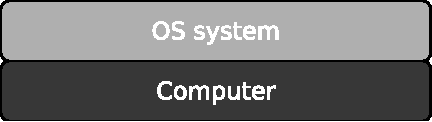
\includegraphics[width=4cm, height=1cm]{images/docker_env_1.pdf}}
\end{textblock*}
\begin{textblock*}{10cm}(6cm,4.5cm) % {block width} (coords)
\onslide<4-4>{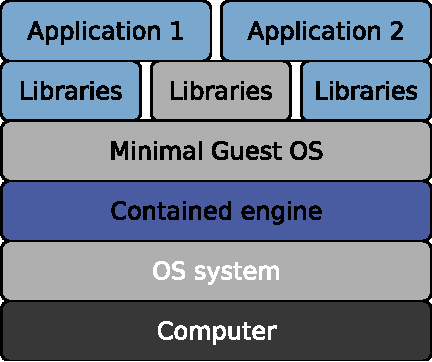
\includegraphics[width=4cm, height=3.7cm]{images/docker_env_2.pdf}} 
\end{textblock*}
\begin{textblock*}{10cm}(8cm,3cm) % {block width} (coords)
\onslide<6-6>{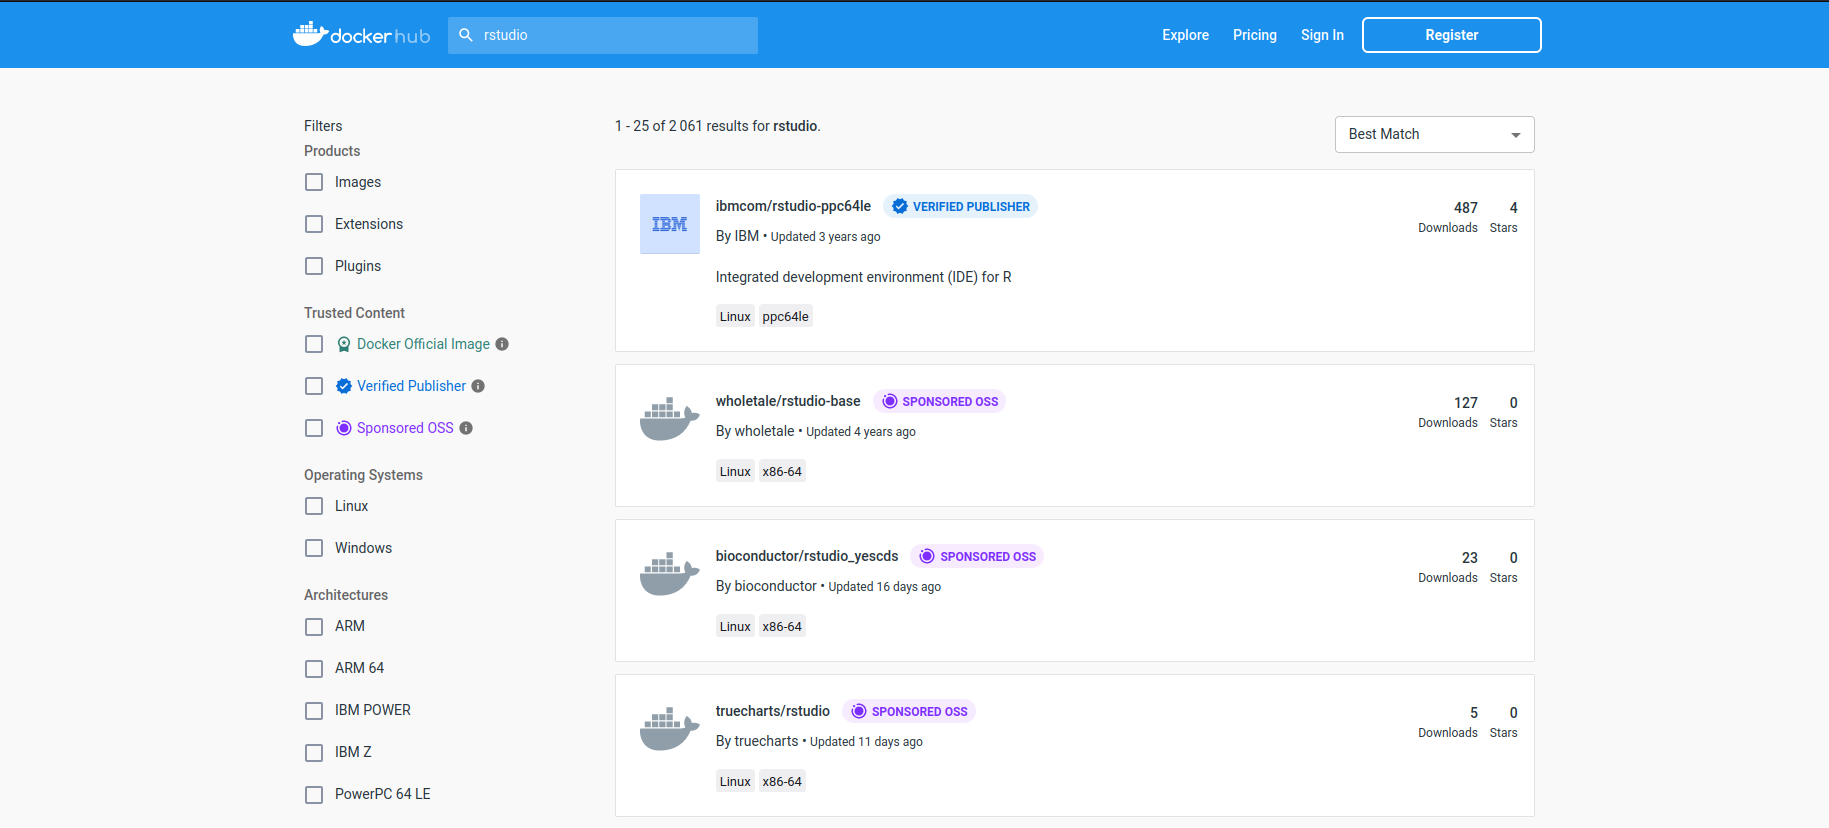
\includegraphics[width=0.9\textwidth]{images/docker_hub.png}}
\end{textblock*}
\begin{textblock*}{10cm}(8cm,3cm) % {block width} (coords)
\onslide<7-7>{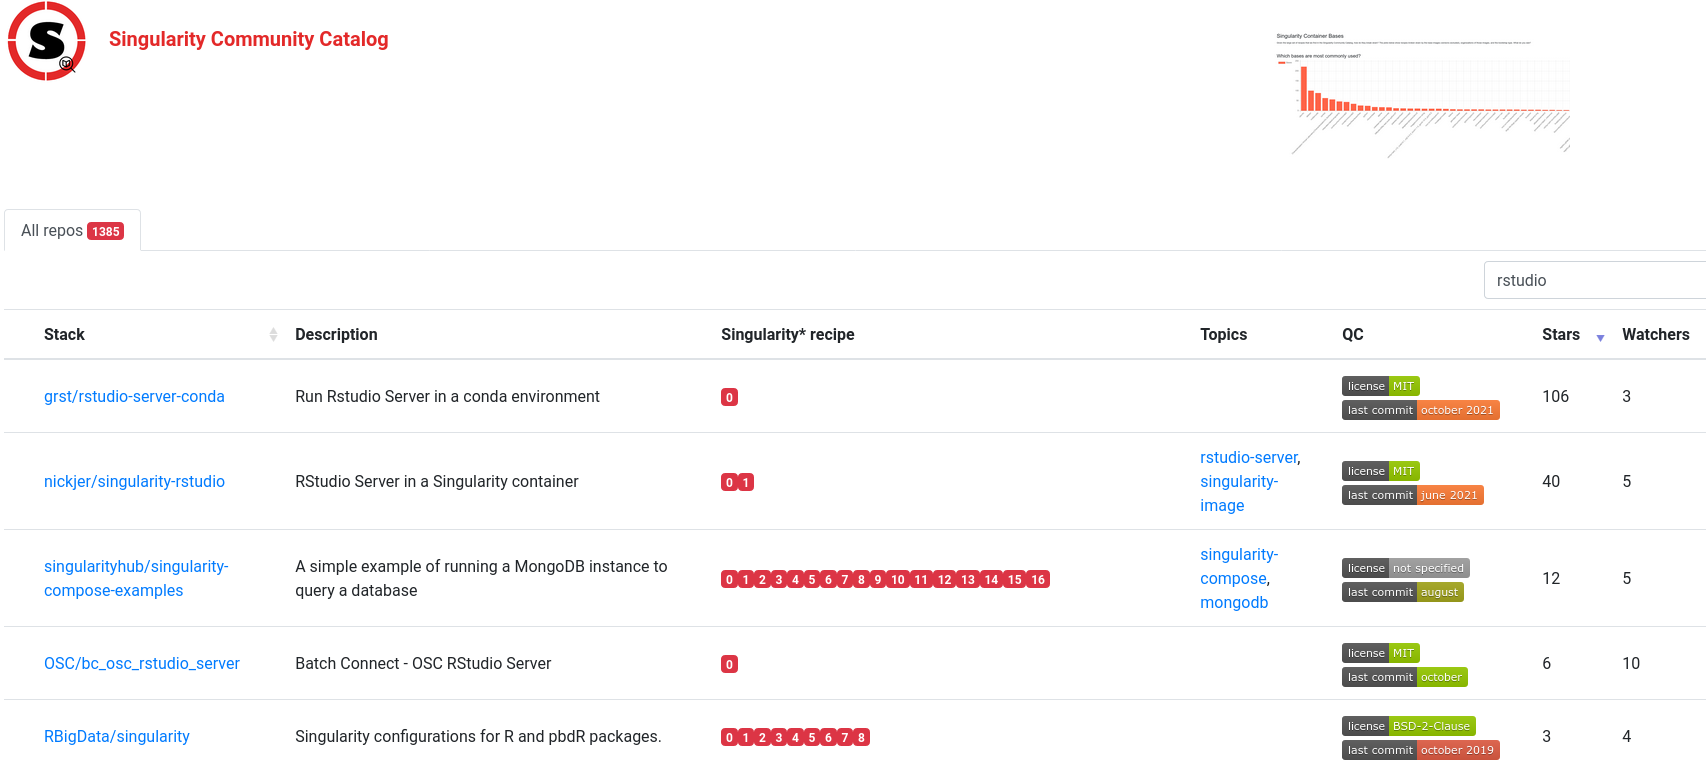
\includegraphics[width=0.9\textwidth]{images/singularity_hub.png}}
\end{textblock*}
\begin{textblock*}{10cm}(0.4cm,1cm) % {block width} (coords)
\onslide<8->{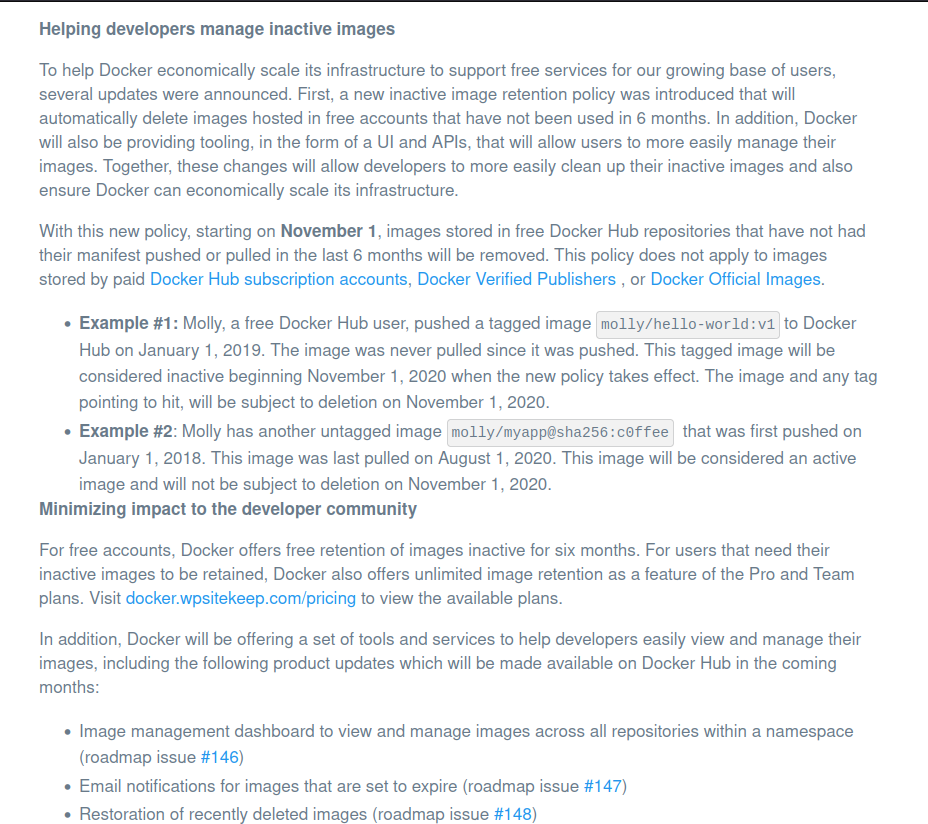
\includegraphics[width=0.8\textwidth]{images/docker_retention.png}}\onslide<8->{\footnote{\url{https://www.docker.com/blog/scaling-docker-to-serve-millions-more-developers-network-egress/}}}
\end{textblock*}

\end{frame}